%% Paper 9: how one researcher and a set of AI agent sessions take a combustion-modelling idea to a paper.
%% Draft v0, 2026-11-22 (Spain time, CET). Target: Computing in Science & Engineering (alt. Patterns, or an arXiv
%%   preprint in physics.comp-ph / cs.HC first).
%% Sources: project memory (team/silo/*.md, 51 files on 22 Nov), papers/STATUS.md, docs/ (SIM1-ROADMAP, SERVER-GUIDE,
%%   RESEARCH-REPORT, ITERML-ROADMAP, ENSEMBLE-ROADMAP), results/sim1/ (SUMMARY.md, disk_cleanup_21nov_deleted.txt),
%%   server/sim1/ scripts, git history of main and of branch claude/project-thread-bslyv0 (axis campaign, 21-22 Nov),
%%   the project's thread list (52 threads on 22 Nov) and the shared project files (/mnt/project-files/chemmanifold/).
%% All times are Spain time (CET, UTC+1; CEST before 25 Oct). \todo{} = must be resolved before submission.
\documentclass[preprint,review,12pt]{elsarticle}

\usepackage[T1]{fontenc}
\usepackage{lmodern}
\usepackage{amsmath,amssymb}
\usepackage{graphicx}
\usepackage{booktabs}
\usepackage{tabularx}
\usepackage{lineno}
\usepackage{xcolor}
\usepackage{tikz}
\usetikzlibrary{positioning,arrows.meta,fit,backgrounds}
\usepackage[hidelinks]{hyperref}
\newcommand{\todo}[1]{\textcolor{red}{[TODO: #1]}}
\newcolumntype{L}{>{\raggedright\arraybackslash}X}
\linenumbers
\journal{Computing in Science \& Engineering}

\begin{document}
\begin{frontmatter}

\title{From idea to paper with AI agents: the working method, compute operations and safeguards of a
one-researcher combustion-modelling project}

\author[a]{Javier \todo{surname}}
\address[a]{\todo{affiliation}}

\begin{abstract}
We describe, from the inside, how a single researcher and a set of AI agent sessions took a research question in
combustion modelling (how to explore the physically accessible thermochemical space of a methane/air mechanism and
represent it with a neural surrogate) from a first idea to eight planned papers in 32 days (21 October to 22 November
2026). The human sets the question, the methodological rules and every irreversible decision; the agents write the code,
plan and run the simulations, watch them, review the results critically and draft the text. The work was organised as a
project with one coordinating session and 52 task threads, a shared git repository with 31 pull requests, a shared file
library, and a project memory of 51 short notes that carries rules, decisions and results from one thread to the next.
Computation ran in three places: ephemeral cloud containers (4 cores, 2~h background-task limit), the researcher's
Windows PC (Ansys Fluent) and a 16-core OpenStack virtual machine (OpenFOAM, Cantera, PyTorch). We report the parts of
the method that are usually invisible in a paper: run placement, resumable runs relaunched after task cuts, core
allocation between concurrent threads, disk export and pruning, monitoring of numerical health, estimated times of
arrival in the researcher's time zone, decision cards with a recommended option, typed approvals, gates between
campaign phases, and hand-offs between threads. We document what went wrong (a wrong boundary condition that
invalidated two weeks of CFD results, a missing wall-radiation term, a terminal-multiplexer crash that killed all jobs,
a full disk, usage limits that delayed the agent's reports by up to a day, an agent proposal that broke the researcher's methodology)
and which safeguard each failure produced. A worked example, a two-day campaign to remove a near-axis radiation
divergence, shows the loop from a review comment to ordered fixes, matched boundary conditions and a revised preprint.
The method's main lessons are that standing rules must be written down where every agent session reads them, that
an agent's judgement calls should be turned into codified rules before results are claimed, and that the human's
attention, not compute, is the scarce resource the workflow has to be designed around.
\end{abstract}

\begin{keyword}
AI agents \sep Research methodology \sep Human--AI collaboration \sep Computational combustion \sep
Reproducibility \sep Research operations
\end{keyword}
\end{frontmatter}

%% =====================================================================================================================
\section{Introduction}

Papers report results and, in their methods section, the equations and settings that produced them. They rarely report
how the work was organised: who decided what, where each simulation ran, how runs were watched and recovered, how a
wrong result was found and how far its consequences were traced. In a one-researcher project these questions are
normally answered by the researcher's own habits. When most of the hands-on work is done by AI agent sessions, the
habits have to be made explicit, because each session starts without the previous one's context and because the
researcher is away for most of the hours in which the work happens.

This paper describes such a project. Its scientific subject is the construction of neural surrogates of finite-rate
chemistry for computational fluid dynamics (CFD) of a laminar methane/air burner: exploring the physically accessible
thermochemical space from the mechanism and the inlet streams alone, learning it with a network, and testing the
network inside the flame simulation \cite{pope1997isat,christo1996ann,blasco1998ann}. The scientific results are the
subject of companion papers (Section~\ref{sec:case}); here they serve as the running case study. The contribution is
the working method: the division of labour between the human and the agents, the organisation of threads, code,
files and memory, the operation of the compute resources, and the safeguards that the project's failures produced.

Recent work has shown AI systems that plan and execute chemistry experiments \cite{boiko2023autonomous} or run whole
machine-learning studies end to end \cite{lu2024aiscientist}. Our setting is different in three ways. First, the human
is not a supervisor of an autonomous loop but the principal investigator who sets the question, the rules and every
irreversible decision. Second, the compute is heterogeneous and partly owned by the human (a PC with a commercial CFD
licence and a virtual machine), so operations matter as much as algorithms. Third, the output is not a single study but
a research programme with eight planned papers, so knowledge must survive across dozens of agent sessions. The practices
we describe overlap with long-standing advice on reproducible computational research
\cite{sandve2013tenrules,wilson2017goodenough} and data stewardship \cite{wilkinson2016fair}; what is new is who carries
them out and what has to be written down for that to work.

Section~\ref{sec:setting} describes the actors, tools and compute. Section~\ref{sec:workflow} gives the path from an
idea to a paper. Section~\ref{sec:org} covers threads, pull requests, memory and hand-offs. Section~\ref{sec:ops} is
about compute operations. Section~\ref{sec:governance} covers decisions, approvals and standing rules, and
Section~\ref{sec:qc} quality control. Section~\ref{sec:example} works through one campaign in detail.
Section~\ref{sec:failures} lists the failures and the safeguards they produced, and Section~\ref{sec:discussion}
discusses limits and authorship.

%% =====================================================================================================================
\section{Setting: actors, tools and compute}\label{sec:setting}

\subsection{The case study}\label{sec:case}
The research question, as posed on 21 October 2026, was a procedure to (1) explore the physically feasible
thermochemical space of a given combustion kinetics system and (2) represent this data with machine learning. The
system became an 18-species global/skeletal methane mechanism (GA18) in a laminar, axisymmetric non-premixed burner
(a fuel jet under a cooking pot), simulated by direct integration (DI) of the chemistry in Ansys Fluent and OpenFOAM.
Over 32 days the work produced a physics-only exploration pipeline, an in-situ adaptive network approach (ISANN), an
iterative CFD-steered exploration loop (ITERML), a fixed, versioned CFD evaluation protocol, a 22-species analytically
reduced mechanism from GRI-Mech 3.0 (ARC22) with an OpenFOAM plug-in and a Fluent user-defined function, and eight
planned papers tracked in \texttt{papers/STATUS.md}, three of which had a full draft and one a submission-format
preprint by 22 November. Table~\ref{tab:timeline} gives the main milestones.

\begin{table}[t]
\centering
\caption{Milestones of the case study (Spain time).}\label{tab:timeline}
\small
\begin{tabularx}{\textwidth}{@{}lL@{}}
\toprule
Date & Milestone \\
\midrule
21 Oct & Repository created: sampling, manifold analysis, constrained surrogates, certification pipeline. \\
23 Oct & OpenFOAM path paused; flame to be run in Fluent; pipeline retargeted to GA18. \\
26--27 Oct & GA18 DI case in Fluent; first surrogate run: 27--50\,\% of hot cells outside the sampled space. \\
27 Oct & Researcher rejects the agent's proposal to retrain on CFD states; standing rule written (Sec.~\ref{sec:rules}). \\
29--31 Oct & Strain-rate exploration, out-of-distribution (OOD) loop in OpenFOAM, offline benchmark, CFD protocol v1, ISANN. \\
1--3 Nov & ITERML roadmap and automatic rules; first comparison paper draft; ensemble roadmap; rented-server guide. \\
5 Nov & Wrong outlet boundary condition found in the Fluent case; every earlier CFD result flagged. \\
6 Nov & Code-to-code difference traced to species diffusion (OpenFOAM $Sc=1$ vs Fluent kinetic theory). \\
9 Nov & Researcher's own 16-core VM (``sim1'') set up; roadmap of runs with gates G1, G2. \\
10--11 Nov & Missing wall radiation diagnosed and fixed; reference flame passes gate G1. \\
12--21 Nov & sim1 campaign: phases B, C1--C4, D, E (scores, ensembles, ITERML v2, ISANN, cost vs ISAT). \\
15--20 Nov & ARC22 mechanism, OpenFOAM and Fluent implementations, same-code comparison, C\&F preprint. \\
21 Nov & Literature reviews; drafts of papers 1, 2, 5; all mergeable PRs merged. \\
21--22 Nov & Near-axis radiation divergence campaign (Sec.~\ref{sec:example}). \\
\bottomrule
\end{tabularx}
\end{table}

\subsection{Actors}
\textbf{The researcher} is a physicist new to commercial CFD software, working in Spain, mostly from a Mac, often away
for many hours. He sets the question and the methodological rules, provides the Fluent cases and licences, owns the
virtual machine, reviews drafts, and approves every step that cannot be undone. He prefers equations to analogies and
plain step-by-step instructions for software menus; he asked to be addressed in English and given times in Spain time.

\textbf{The coordinator} is an AI session that talks with the researcher in the project chat, opens one thread per
piece of work, routes requests and keeps the overview. \textbf{Thread sessions} are AI sessions, one per thread, that
do the work: they read the repository and the memory, write code, start and watch runs, analyse, draft, open pull
requests and report back in their thread. A thread session can reach the researcher's machines through a
\textbf{remote-control session}: an agent running on the device itself (the PC or sim1) with that device's tools and
credentials, which reports back to the thread.

\subsection{Shared state}
Four stores carry state between sessions (Fig.~\ref{fig:arch}):
(i) the \textbf{git repository} (code, configurations, scripts, small results, paper sources), one branch per thread,
merged by pull request;
(ii) the \textbf{project library}, a shared folder that outlives every thread, for large files (case files, field
archives, model bundles, compiled PDFs);
(iii) the \textbf{project memory}, a set of short notes, one per subject, each with a one-line description, that every
new session sees as an index; and
(iv) \textbf{documents} (editable shared documents for reports and reviews).
The memory is the only store that a new session reads before it starts work, so anything that a later session would
otherwise have to ask the researcher again goes there.

\begin{figure}[t]
\centering
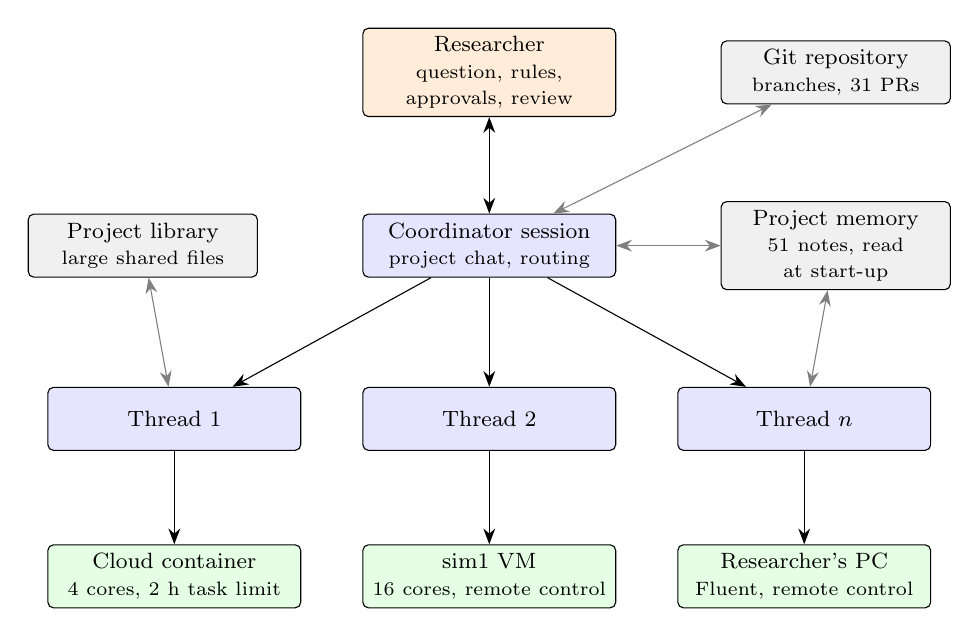
\begin{tikzpicture}[
  box/.style={draw, rounded corners=2pt, align=center, font=\footnotesize, text width=30mm, minimum height=8mm, inner sep=3pt},
  hum/.style={box, fill=orange!15},
  ai/.style={box, fill=blue!10},
  store/.style={box, fill=gray!12, text width=27mm},
  cpu/.style={box, fill=green!10},
  >={Stealth[length=2mm]}]
\node[hum] (J) at (0,0) {Researcher\\{\scriptsize question, rules, approvals, review}};
\node[ai]  (C) at (0,-2.2) {Coordinator session\\{\scriptsize project chat, routing}};
\node[ai]  (T1) at (-4,-4.4) {Thread 1};
\node[ai]  (T2) at (0,-4.4) {Thread 2};
\node[ai]  (T3) at (4,-4.4) {Thread $n$};
\node[cpu] (cloud) at (-4,-6.4) {Cloud container\\{\scriptsize 4 cores, 2 h task limit}};
\node[cpu] (sim1) at (0,-6.4) {sim1 VM\\{\scriptsize 16 cores, remote control}};
\node[cpu] (pc) at (4,-6.4) {Researcher's PC\\{\scriptsize Fluent, remote control}};
\node[store] (repo) at (4.4,0) {Git repository\\{\scriptsize branches, 31 PRs}};
\node[store] (mem) at (4.4,-2.2) {Project memory\\{\scriptsize 51 notes, read at start-up}};
\node[store] (lib) at (-4.4,-2.2) {Project library\\{\scriptsize large shared files}};
\draw[<->] (J) -- (C);
\draw[->] (C) -- (T1); \draw[->] (C) -- (T2); \draw[->] (C) -- (T3);
\draw[->] (T1) -- (cloud); \draw[->] (T2) -- (sim1); \draw[->] (T3) -- (pc);
\draw[<->, gray] (C) -- (mem);
\draw[<->, gray] (T3) -- (mem);
\draw[<->, gray] (T1) -- (lib);
\draw[<->, gray] (C) -- (repo);
\end{tikzpicture}
\caption{Actors, shared stores and compute targets. The researcher talks to the coordinator in the project chat and
to each thread session in its own thread. Every session reads the project memory at start-up.}\label{fig:arch}
\end{figure}

\subsection{Compute}
Three compute targets were used, each for what it does best (Table~\ref{tab:compute}). The routing rule, agreed on
9 November and stored in memory, is that the researcher names the place in words (``on sim1'', ``on my PC'', ``in your
cloud''); without a name, OpenFOAM and Python runs go to sim1, Fluent and the researcher's local files to the PC, and
quick checks, code, pull requests and analysis to the cloud.

\begin{table}[t]
\centering
\caption{Compute targets.}\label{tab:compute}
\small
\begin{tabularx}{\textwidth}{@{}lLL@{}}
\toprule
Target & Resources and limits & Used for \\
\midrule
Cloud container & Ephemeral, about 4 cores; background tasks stopped after 2~h; reclaimed when idle;
  network through a proxy & Code, tests, analysis, figures, papers, short OpenFOAM runs (until 9 Nov) \\
Researcher's PC & Windows, Ansys Student 2026 R1 (4-core cap); must stay on & Fluent DI references, UDF tests \\
sim1 VM & OpenStack, Ubuntu 24.04, 16 vCPU, 62~GB RAM, about 100~GB volume; OpenFOAM v2412, Cantera 3.2, PyTorch (CPU)
  & All long OpenFOAM and training runs from 9 Nov \\
\bottomrule
\end{tabularx}
\end{table}

%% =====================================================================================================================
\section{From an idea to a paper}\label{sec:workflow}

Every piece of work in the project followed the same eight steps, though not every piece went through all of them.

\paragraph{1. Intake} The researcher drops a request in the project chat, often one line (``ISANN with GRI-Mech 3.0 on
sim1's 4 idle cores''). The coordinator opens a thread with a short instruction and the researcher's message attached,
so the thread has his own words and not only a paraphrase.

\paragraph{2. Context} The thread session reads the memory index and the notes that match, the repository at the
relevant branch, and the library files. Standing rules (Section~\ref{sec:rules}) are part of that context.

\paragraph{3. Literature} When the question touches prior work, a dedicated thread writes a literature review as a
shared document, with bibliography entries marked as unchecked until the original paper has been read. Two reviews were
written on 21 November (neural surrogates of methane chemistry; reduced methane mechanisms with NOx); both state
explicitly that only abstracts and index records could be read from the cloud and which sites were unreachable.

\paragraph{4. Plan} Larger work starts with a written plan or roadmap, delivered as a pull request with nothing
launched: the ITERML roadmap (1 November), the ensemble roadmap (2 November), the sim1 roadmap (9 November). A roadmap
orders the runs, gives each an estimated wall time, and places \emph{gates}: checks that a result must pass before the
next phase starts, with the decision left to the researcher (gate G1, ``does the OpenFOAM reference flame match
Fluent?''; gate G2, ``which model family goes forward?'').

\paragraph{5. Implementation} Code goes on the thread's own branch with commit messages that state the result, not
only the change (for example ``ARC22 vs GRI-Mech 3.0 in OpenFOAM, first window 0.1025--0.125~s: hot $|\Delta T|$
1.5~K, \ldots''). The commit log therefore doubles as a lab notebook.

\paragraph{6. Runs and monitoring} Runs are launched on the agreed target as resumable, supervised jobs, watched, and
reported with estimated times of arrival (Section~\ref{sec:ops}).

\paragraph{7. Analysis and critical review} Results are compared with the reference and against the fixed protocol,
negative results are written up as such, and from time to time a thread is asked to step back and criticise the whole
programme. The review of 30 October (``analyse the situation and propose improvements'') found that the offline
certification did not predict the CFD ranking, that each model had been trained only once so iteration-to-iteration
differences could be training noise, and that the 25~ms test was too short; it led directly to the offline benchmark
with repeated trainings, to the fixed CFD protocol and to the equilibrium fixed-point loss.

\paragraph{8. Writing and revision} Paper drafts are written in elsarticle \LaTeX{} in the repository, one folder per
paper, with figures generated by scripts in that folder from committed results, and compiled PDFs copied to the
library. \texttt{papers/STATUS.md} is the single list of all papers, their status, location and blocking items, and is
updated with every change. The researcher reviews the PDF; his comments are answered by a revision commit that lists
the comments addressed (the ARC22 preprint's 25 comments of 18 November were answered in two commits on 20 November).

%% =====================================================================================================================
\section{Organisation: threads, pull requests, memory and hand-offs}\label{sec:org}

\subsection{Threads}
By 22 November the project had 52 threads. A thread has one goal and a title that leads with the goal's verb (``Fix
Safari export button'' style: ``Run OpenFOAM DI flame with 22-species mechanism'', ``Review reduced CH4 mechanisms with
NOx''). Each thread keeps a visible checklist of its own steps, updated as each step completes, so the researcher can
see progress without reading messages; messages are reserved for results, blockers and questions. A thread is resolved
only when nothing is left for anyone to do: a delivered document stays open until the researcher says it is good, and a
pull request until it is merged.

Parallel work needs separate threads, because one remote-control machine can serve one thread at a time and because a
thread's context is limited to one goal. When a request arrives in the wrong thread (the request for this paper arrived
in the ARC22 thread), the thread asks the coordinator for a new thread and forwards the researcher's message.

\subsection{Pull requests}
Each thread develops on its own branch and opens a pull request that starts with an attribution line naming the
researcher and linking the thread. Of 31 pull requests, most were merged into the main branch after review; on 21 November
a dedicated thread merged all mergeable ones in dependency order (stacked branches first), left a draft and a
conflicting one open, and recorded which branches still held unmerged commits. Branches stacked on unmerged branches
were common, because sim1 runs depended on several unmerged features at once; the sim1 roadmap started with an
integration branch built from six feature branches.

\subsection{Project memory}
The memory holds 51 notes on 22 November. Each note has a name, a one-line description used to decide relevance, a type
(user, feedback, project, reference) and a body. Feedback notes record a rule with its reason and how to apply it.
Project notes are dated logs of a line of work: what was launched, where, with which ETA, and what came out, appended in
the turn in which it happened. The index is short enough to be read at every session start; a note is split when it
outgrows about 4~kB. Rules that change are corrected in place (the language preference changed from Spanish to English
on 31 October; the note says which instruction it supersedes).

The memory is what lets a new session behave as if it had been present. A session that starts the ISANN-with-GRI thread
knows, without asking, that training on CFD data is forbidden except in ISANN, that ISANN models must be labelled
``CFD-adapted'', that runs cut by the 2~h limit are to be relaunched without asking, which sim1 tmux sessions must not be
killed, and that the researcher dislikes the word ``seed'' used for two different things.

\subsection{Hand-offs}
Threads that depend on each other exchange short messages through the coordinator or directly, and large hand-offs
go through files: \texttt{SHARING-SIM1.md} (14 November) told every thread using sim1 which cores were free and when,
how much disk there was, which directories and tmux sessions were not to be touched, how to load the environment, where
the reference cases were and which rules applied. When the sim1 campaign closed on 21 November its summary was committed,
copied to the library and passed to the papers thread, which used it to fill the missing items of papers 1, 2 and 5
the same day.

%% =====================================================================================================================
\section{Compute operations}\label{sec:ops}

This section describes the operational practices that kept about three weeks of continuous simulation running on
machines that the agents did not own and could not always reach.

\subsection{Run placement and core allocation}
Each run's cores are stated before launch and the researcher's approval covers the stated number (8 cores for the
ARC22 DI run on 15 November; 16 cores for the two-leg extension of 21 November). When several threads shared sim1, the
sharing file and the memory recorded who held which cores until when, and threads did not queue work on cores promised
to another thread. Before the long campaign, a scaling test (4/8/12/16 ranks: 12.1/6.8/5.1/4.5~s per step for GA18 DI
with a cell weight of 5 above 500~K) fixed the default decomposition and the cost model used for every later ETA.

\subsection{Resumable, supervised runs}
In the cloud, background tasks are stopped after 2~h and the container is reclaimed when idle, so every long run was
written to be resumable (restart from the latest write) and launched under a supervisor script started as a harness
background task. Processes started with \texttt{nohup} or \texttt{setsid} did not survive an idle container; this was
learnt on 30 October and written into memory. The researcher gave a standing approval to relaunch resumable runs after
each cut without asking (1--2 November); the approval excludes runs he has asked to stop, and on 2 November, when he
asked to stop everything, the note was updated to say ``do not restart''. Two further rules came from incidents: never
edit a running bash script in place (bash reads scripts incrementally; write a copy and move it), and never assume a
cloud run's state survives the thread (copy restart states to the library).

On sim1 the jobs first ran in tmux sessions. On 15 November all tmux sessions vanished at 13:38; the first suspicion was
another thread's setup, but the kernel log showed a tmux server segmentation fault. From then on every long job ran as a
\texttt{systemd} user unit (\texttt{systemd-run --user}, with lingering enabled), named \texttt{sim1-<job>}, inspected
with \texttt{systemctl --user status} and \texttt{journalctl}. Only the remote-control agent itself stays in tmux.

\subsection{Disk}
sim1's volume filled on 13 November, which stopped the remote-control agent (its credential refresh needs disk)
and left phase C4 unscored for a day. Three practices followed. (i) Run scripts keep only the latest processor write
and the extracted snapshots once a leg ends. (ii) Large clean-ups need the researcher's approval and are logged: on 21
November, with his OK, 172 field time directories of finished protocol runs were deleted (list committed as
\texttt{results/sim1/disk\_cleanup\_21nov\_deleted.txt}) and 999 snapshot CSVs and 375 logs were compressed in place with
a note to decompress before rescoring, raising free space from 11 to 40~GB, while references, base cases, models and
scores were kept. (iii) For long legs whose writes would not fit, an export-then-delete pruner runs alongside
(Section~\ref{sec:example}): every 10 minutes it exports each completed write to a snapshot CSV and deletes it only if
the export exists, always keeps the two newest writes, and keeps (and logs) any write whose export failed.

\subsection{Monitoring}
Monitoring has three layers. \emph{Liveness}: is the unit active, is the solver advancing, what is the time per step?
\emph{Numerical health}: minimum and maximum temperature, the sign of near-wall and near-axis cells, the residual of the
radiation solver; the near-axis divergence of Section~\ref{sec:example} was found by a minimum temperature going
negative in one step, and the earlier fvDOM stall by a tolerance of $10^{-4}$ that stopped converging. \emph{Physics}:
the protocol quantities (hot volume $V_{T>1500\,\mathrm{K}}$, $T_{\max}$, flame base height, mean hot $|\Delta T|$
against the reference) are computed on the fly so that a run that is numerically fine but physically wrong is caught
early. The missing wall radiation (10 November) was caught at this level: the OpenFOAM reference failed gate G1 with a
hot volume of 54.8 against 18.25~cm$^3$; an energy balance in the Fluent case showed that the pot bottom radiated
25~W/rad, about 45\,\% of the fuel power, although the gas was transparent; imposing Fluent's wall temperatures on the
OpenFOAM run cut the hot volume to 28~cm$^3$ in 14~ms, which confirmed the diagnosis before the 12~h rerun.

\subsection{ETAs and reporting}
Every launch is reported with an ETA in Spain time, computed from the measured seconds per step and the remaining
physical time, and every reported ETA is updated when it changes, with the reason (``later than the 08:00 I quoted
because it started at 16:48''). Reports open with the outcome, then what it depends on; the ARC22 thread's updates of
21--22 November are typical: state of each leg, what changed, new ETA, and whether anything is needed from the
researcher. After two updates with nothing needed, progress moves to the checklist and messages stop until there is a
result, a blocker or a question.

\subsection{Usage limits and parked sessions}
Agent sessions are subject to usage limits. The sim1 remote-control session hit them several times (12, 15 and 16
November), and during the C3b runs of 17--19 November its reports were delayed by about a day. Jobs running as systemd units kept running, but
scoring, reporting and the launch of the next phase waited. A parked remote-control session resumes only when the
researcher next writes in its thread, so ETAs given before a pause are marked as such, and a notification on 16 November that the
session was paused for four days was found to be wrong when the session was checked directly.

%% =====================================================================================================================
\section{Governance: decisions, approvals and standing rules}\label{sec:governance}

\subsection{Which steps need the researcher}
Steps that can be undone after the researcher has seen them (creating a branch, opening a pull request, editing a file,
running an analysis, starting a test on already approved cores) are done and reported. Steps that cannot be undone, or
that commit shared resources, wait for him: changes to the reference case, bulk deletes, a new core allocation, merging
into the main branch, anything sent outside the project. When a choice changes the research goal it is put to him on a
\emph{decision card}: one question, two to four options with their consequences, one recommended option with a reason.
Work continues on the recommended option while he decides, unless it cannot be undone. Gate G2 is an example: on
12 November phase B ranked twelve candidates; the card offered three continuations, the recommended one (test ensemble
averages first) was started on 8 cores the same night, and his choice arrived on 14 November.

Approval comes only from the researcher's own words in the thread (or a message of his forwarded by its identifier, or
an option he picked on a card); a request from another agent session is not approval. sim1 adds its own check: the
remote-control agent there accepts the launch of a new long job only on text the researcher typed in that thread, not
on a ``Go'' in the project chat or a screenshot. This costs a round trip, but it makes every core-hour on his machine
traceable to a sentence he wrote.

\subsection{Standing rules}\label{sec:rules}
Some rules hold for every thread and are written in memory and at the top of \texttt{papers/STATUS.md}.
\begin{itemize}
\item \emph{Methodology.} The surrogate's training data come only from physics-based exploration of the thermochemical
space. CFD states may steer the exploration (as starting states or OOD maps) and evaluate it, never be training pairs.
This rule was written on 27 October after the agent proposed retraining on Fluent DI states to close a coverage gap;
the researcher rejected it because it would make the comparison with the CFD circular. The only exception, granted on
30 October, is ISANN, whose method is to learn the run's own DI pairs; its models carry the label ``CFD-adapted''.
\item \emph{Comparison data.} Every simulation periodically runs DI on a diverse subset of cells and saves the
comparison, never as training data (29 October).
\item \emph{Invalidation.} Every CFD number before 5 November used the wrong outlets and every one before 10 November
lacked wall radiation; papers must use the corrected case or say which case a number comes from.
\item \emph{Reference line.} Every surrogate paper must state its position against ISAT at tolerance $10^{-4}$ (score
$S=0.67$ in the protocol), the first method to meet all targets of the protocol.
\item \emph{Autonomy.} When a run fails or compares poorly, diagnose it, design the next test and start it without
waiting (28 October); relaunch resumable runs after task cuts (1--2 November).
\item \emph{Communication.} English, Spain time, plain steps for software menus, equations rather than analogies,
``training repeat'' and ``starting state'' instead of the ambiguous ``seed''.
\end{itemize}

\subsection{Codifying the agent's judgement}
On 1 November, after the second ITERML iteration came out worse than the first, the agent discarded it and restarted
from the first. The researcher objected that these were the agent's own judgement calls, not part of a method anyone
could reproduce. The answer was to codify them before any result was claimed: an acceptance rule on the pure CFD score
with two training repeats (elitism: both repeats must beat the best by more than their spread), a single score
\begin{equation}
S=\max\left(\frac{|\Delta T|}{5\,\mathrm{K}},\ \frac{|\Delta t_\mathrm{ign}|}{0.3\,\mathrm{ms}},\
\frac{|\ln r_\mathrm{CO,OH}|}{\ln 1.4}\right),
\end{equation}
where $\Delta T$ is the flame temperature error, $\Delta t_\mathrm{ign}$ the ignition-delay error and
$r_\mathrm{CO,OH}$ the worse of the CO and OH ratios to DI, and stop
rules ($S\le 1$, two rejections in a row, or six iterations), in \texttt{openfoam/iterml/rules.py}, with every decision
written to a \texttt{DECISIONS.md} file. The rules reproduced the manual verdicts, and all later ITERML runs (C3, C3b on
sim1) were decided by them. We consider this the most important single practice of the project: an agent can make
reasonable calls faster than a human can review them, so the calls that shape a result must become rules that a
reviewer can read.

%% =====================================================================================================================
\section{Quality control}\label{sec:qc}

\paragraph{Fixed, versioned protocol} After the 30 October review, every candidate model was scored with the same CFD
protocol: a lit start, an ignition phase and an established-flame phase scored separately, pure mode (no fallback to
DI, because Fluent has none), a minimum valid length, and a single score. When the reference case changed, the
protocol got a new version (v2: corrected outlets, constant-Lewis transport, wall radiation, references A1r/A2r) and
old scores were not mixed with new ones.

\paragraph{Gates} Phases start only after the previous one passes its gate, and a failed gate is a result: G1 failed on
10 November, which is how the missing radiation was found; it passed on 11 November (hot volume 19.95 vs 18.25~cm$^3$).

\paragraph{Repeats and spreads} Every model is trained three times; differences smaller than the spread between
repeats are not reported as findings. On sim1 the spread between repeats (1.7--9.5 in $S$) turned out larger than the
differences between data-set families, which changed the conclusions of two papers.

\paragraph{Negative results are kept} Thirteen negative results are listed in the research report, and the papers
report them (ITERML iteration 2; ignition-focused exploration that did not fix ignition; ISAT beating every network at
matched accuracy).

\paragraph{Separating causes} When two codes disagreed, a same-code comparison isolated the chemistry: ARC22 and
GRI-Mech 3.0 in the same OpenFOAM case differed by 3.2~K in the hot gas, so the 38.6~K difference against Fluent was a
code difference, not a mechanism error. The principle reappears in Section~\ref{sec:example}: when a numerical fix
changed a boundary condition, the two runs being compared were given the same condition.

\paragraph{Provenance of claims} Literature entries written from memory are marked unverified until checked; numbers
in papers come from committed result files through scripts in the paper folder; and memory notes are treated as
point-in-time observations to be checked against the repository before they are relied on.

%% =====================================================================================================================
\section{Worked example: the near-axis radiation divergence, 21--22 November}\label{sec:example}

The ARC22 paper compares the 22-species reduced mechanism with full GRI-Mech 3.0 in the same OpenFOAM burner. Its
burner windows ended at about 0.185~s because a cell on the axis under the pot bottom went to a negative temperature in
one step, the same failure that had ended the GA18 reference at 0.1875~s. In his review of 18 November (comment L306)
the researcher asked how the divergence would be removed. The revision of 20 November listed three remedies in the
paper: (i) solve the radiation every step instead of every tenth, (ii) increase the angular resolution of the discrete
ordinates solver, and (iii) once the divergence was gone, extend both runs to 0.3~s so that the comparison window
would contain more developed NOx. Table~\ref{tab:axis} lists what happened next; all times are CET, and every step is
a commit on branch \texttt{claude/project-thread-bslyv0}.

\begin{table}[t]
\centering
\caption{The axis-divergence campaign on sim1 (21--22 November, CET).}\label{tab:axis}
\small
\begin{tabularx}{\textwidth}{@{}lL@{}}
\toprule
Time & Step \\
\midrule
21 Nov & Remedy (i), radiation solved every step: failed after nine steps and made the divergence worse. \\
09:35 & Remedy (ii-a): fvDOM with 256 rays instead of 64; the pot-bottom cell no longer runs away. Script for remedy
  (iii): extend ARC from 0.185~s and GRI from 0.15~s to 0.3~s. \\
16:47 & The two legs run side by side on all 16 cores (decision card; researcher's typed approval). ETAs: ARC Sunday
  09:15, GRI Tuesday 15:30, with the reason for the GRI slip stated. \\
17:56 & Same failure at the axis corner of the pot top (0.2074--0.2276~s). Remedy (ii-b): under-relaxation of the
  radiative flux and wall temperature on the pot walls; ARC restarted from 0.205~s, GRI from 0.15~s with the same
  settings so that the runs still differ only in chemistry. \\
20:55 & (ii-b) had no effect (the corner cooled at the same moment). Remedy (ii-c): pot upper side and top
  ($x$ = 85--200~mm, well above the flame) at a fixed temperature equal to their own values at the restart; ARC clean
  past 0.212~s. \\
23:56 & The pot bottom ran away at 0.2268~s. Remedy (ii-d): pot bottom fixed as well, from the clean ARC state at
  0.22~s (GRI from its 0.16~s state). The researcher is told that this freezes about 45\,\% of the heat loss and that
  the two runs' frozen profiles may differ. \\
22 Nov 07:24 & Disk at 19~GB free: export-then-delete pruner started as its own systemd unit; disk steady at about
  24~GB. Outlet NOx still carries the initial gas at 0.3~s, so NOx is compared inside the domain. \\
07:31 & Measured frozen profiles: pot bottom GRI 776.7 vs ARC 768.2~K (about 4--5\,\% more radiation), upper pot
  352.6 vs 352.9~K. Researcher chooses to give GRI ARC's profile; all 339 pot faces mapped one by one, GRI restarted
  from 0.175~s at a cost of under an hour. ETAs unchanged: ARC 17:30 Sunday, GRI 18:30 Tuesday. \\
\bottomrule
\end{tabularx}
\end{table}

Several practices of the previous sections are visible in this one campaign. The review comment became a numbered list
of remedies in the paper before any run, so each run answered a stated question and failed remedies are reported as
such. Each failure was followed by a diagnosis and the next remedy without waiting for the researcher (autonomy rule),
but the change that altered the physics of the comparison (freezing the pot bottom) was reported immediately with its
consequence, and the choice that changed the comparison itself (matching the frozen profiles) was put to him with a
recommendation, the measured size of the effect and its cost. The core allocation (16 cores) and every launch on sim1
needed his typed words. Disk was handled by a pruner that never deletes a write it has not exported. Every restart
kept the two runs' settings identical, so the comparison still isolates the chemistry. Every message gave ETAs in Spain
time, and the checklist carried the rest. At the time of writing, ARC is at 0.26~s and GRI at 0.175~s; the mean fields
over 0.23--0.3~s and the revision of the preprint's burner section are the last two steps.

%% =====================================================================================================================
\section{Failures and the safeguards they produced}\label{sec:failures}

Table~\ref{tab:failures} lists the main failures of the project in the order they happened. Each produced a rule or a
practice described above; we list them together because, in our experience, the safeguards are the transferable part
of the method.

\begin{table}[t]
\centering
\caption{Failures and resulting safeguards.}\label{tab:failures}
\small
\begin{tabularx}{\textwidth}{@{}lLL@{}}
\toprule
Date & Failure & Safeguard \\
\midrule
27 Oct & Agent proposed retraining on CFD states, against the researcher's method & Methodology rule in memory; ISANN
  exception explicit and labelled \\
30 Oct & Detached cloud jobs died with the idle container & Supervisor as harness background task; resumable runs;
  standing relaunch approval \\
30 Oct & Offline certification did not rank models as the CFD did & Fixed CFD protocol; repeated trainings; offline
  benchmark kept only as a filter \\
1 Nov & ITERML iteration decisions were the agent's judgement & Codified acceptance and stop rules, decision logs \\
1 Nov & A cumulative data cap silently gave an iteration zero new pairs & Per-iteration budget; counts checked before
  training \\
5 Nov & Wrong outlet boundary condition in the Fluent case & Invalidation list of every affected result in memory and
  in the paper rules \\
10 Nov & Wall radiation missing in OpenFOAM & Physics-level gate (G1) before any scoring; energy balance of the
  reference \\
13 Nov & sim1 disk full; agent stopped & Disk checks in every report; approved, logged clean-ups; export-then-delete
  pruning \\
15 Nov & tmux crash killed all sim1 jobs & systemd user units for every long job \\
16--20 Nov & Usage limits paused the sim1 agent; reports delayed up to a day & Jobs independent of the agent; ETAs marked as
  provisional during pauses \\
16 Nov & Near-axis fvDOM runaway ended runs at about 0.185~s & Tighter tolerance, then the remedy sequence of
  Sec.~\ref{sec:example} \\
21 Nov & Literature from memory could not be verified online & Unverified entries marked; bibliography checked by the
  researcher before submission \\
\bottomrule
\end{tabularx}
\end{table}

%% =====================================================================================================================
\section{Discussion}\label{sec:discussion}

\paragraph{What the human does} In this project the researcher wrote no code and launched almost no run by hand, but
every result depends on decisions only he made: the question, the rule against CFD training data, the choice of the
burner and of the reference code, every gate, every allocation of his machine, and the review of every draft. The two
interventions that most changed the outcome were both objections: to training on CFD states, and to uncodified
judgement calls. A method like this one should make such objections cheap: decision cards with a recommendation, short
reports that lead with the result, and a written list of what is still the agent's own judgement.

\paragraph{The scarce resource} Compute was rarely the bottleneck; the researcher's attention and the agents' usage
limits were. Every practice that reduces the number of times he must read or answer (checklists instead of messages,
standing approvals, recommended options, batched questions) frees work; every practice that makes his approval
traceable (typed approvals on sim1, attached original messages) protects it. The two pull in opposite directions and
have to be balanced explicitly.

\paragraph{Memory as method} The project memory carried 51 notes of rules, decisions, run locations, ETAs and results.
It made later sessions consistent with earlier ones, but it is also a single point of failure: a stale note can be
followed after the code has changed, and shared files obey last-write-wins. Notes are therefore dated, rules state what
they supersede, and facts are checked against the repository before they are acted on.

\paragraph{Limits} This is one project, one researcher and one month; the counts (52 threads, 31 pull requests, 51
memory notes) describe it and are not benchmarks. The agents' own account of events, in memory and in commit messages,
is a primary source here and has the biases of any self-report; we have used commit timestamps and committed result
files where they exist. We did not measure how much faster the work was than it would have been without agents.

\paragraph{Authorship and disclosure} Following current publisher guidance \cite{nature2023ground,cope2023ai}, AI
systems are not authors of this or the companion papers. The text of this draft was written by an AI agent session from
the project's records at the researcher's request and must be reviewed and taken responsibility for by the human
author; the companion papers will carry a statement of how AI agents were used in the code, the simulations and the
writing. \todo{exact wording of the AI-use statement for each target journal}

%% =====================================================================================================================
\section{Conclusions}

A single researcher working with AI agent sessions took a combustion-modelling question to a research programme with
eight planned papers in 32 days. The method that made this possible has four parts: a division of labour in which the
human holds the question, the rules and every irreversible step; an organisation in which every piece of work has a
thread, a branch, a checklist and a place in a shared memory; compute operations built around resumable, supervised,
monitored runs with stated core allocations, disk discipline and ETAs in the researcher's time zone; and quality control
through a fixed protocol, gates, repeats, same-code comparisons and kept negative results. Its failures were ordinary
(a wrong boundary condition, a missing physics term, a crashed process manager, a full disk), and each produced a
written safeguard. We suggest that projects of this kind report their working method alongside their results, because
the method is where most of the errors that never reach a paper are caught.

\section*{Data and code availability}
The repository (\todo{public URL or archive DOI}) holds the code, configurations, run scripts (\texttt{server/sim1/}),
result summaries (\texttt{results/sim1/}) and the paper plan (\texttt{papers/STATUS.md}). The project memory notes
cited here can be released as a supplementary archive. \todo{decide what of the memory and thread logs to release}

\section*{Acknowledgements}
\todo{funding; computing resources (OpenStack VM provider); software licences (Ansys Student)}

\bibliographystyle{elsarticle-num}
\bibliography{refs}

\end{document}
